\documentclass[aspectratio=169,10pt]{beamer}

% Encoding, Fonts, and Graphics
\usepackage[utf8]{inputenc}
\usepackage{booktabs}
\usepackage{graphicx}
\usepackage{tikz}
\usepackage[skins]{tcolorbox}

% Theme Customization
\usetheme{Madrid}
\usecolortheme{whale}

% Custom Curated Colors
\definecolor{spaceNavy}{RGB}{11, 27, 61}
\definecolor{darkNavy}{RGB}{6, 16, 38}
\definecolor{electricCyan}{RGB}{0, 168, 150}
\definecolor{lightCyan}{RGB}{236, 250, 248}
\definecolor{goldAccent}{RGB}{210, 155, 20}
\definecolor{lightGold}{RGB}{254, 250, 235}
\definecolor{alertRed}{RGB}{175, 35, 35}
\definecolor{lightRed}{RGB}{253, 240, 240}
\definecolor{cardBg}{RGB}{247, 249, 253}
\definecolor{cardFrame}{RGB}{210, 222, 240}
\definecolor{greenAccent}{RGB}{22, 163, 74}
\definecolor{lightGreen}{RGB}{240, 253, 244}

% Beamer Palette Settings
\setbeamercolor{palette primary}{bg=spaceNavy,fg=white}
\setbeamercolor{palette secondary}{bg=spaceNavy!90,fg=white}
\setbeamercolor{palette tertiary}{bg=darkNavy,fg=white}
\setbeamercolor{title}{bg=spaceNavy,fg=white}
\setbeamercolor{frametitle}{bg=spaceNavy,fg=white}
\setbeamercolor{structure}{fg=spaceNavy}
\setbeamerfont{subtitle}{size=\small,series=\normalfont}

\setbeamertemplate{navigation symbols}{}

% Split Footer: Left (Author), Right (Subtitle) in Subtitle Font Size
\setbeamertemplate{footline}{
  \leavevmode%
  \hbox{%
  \begin{beamercolorbox}[wd=.47\paperwidth,ht=2.8ex,dp=1.1ex,left,leftskip=2ex]{author in head/foot}%
    \small Jason Pandian (\texttt{pandiajason@gmail.com})
  \end{beamercolorbox}%
  \begin{beamercolorbox}[wd=.53\paperwidth,ht=2.8ex,dp=1.1ex,right,rightskip=2ex]{title in head/foot}%
    \small Why Deep Space Breaks Conventional DES Paradigms
  \end{beamercolorbox}}%
  \vskip0pt%
}

% Global tcolorbox settings for slides
\tcbset{
  boxrule=0.7pt,
  arc=2.5pt,
  boxsep=0.5pt,
  left=4pt,
  right=4pt,
  top=1.5pt,
  bottom=1.5pt
}

% Title Metadata
\title[\textbf{Limits of DES in Interplanetary Sim}]{\textbf{The Limits of Discrete-Event Schedulers in Interplanetary Network Simulation}}
\subtitle{Why Deep Space Breaks Conventional DES Paradigms}
\author[\textbf{Jason Pandian}]{\textbf{Jason Pandian} (\textit{Presenter})}
\institute[NIT]{
  Department of Information Technology, Nehru Institute of Technology, Coimbatore, India
}
\date[\textbf{ICNS3 - 2026}]{\textbf{International Conference on ns-3 (ICNS3 - 2026)} $\cdot$ Lightning Talk}

\begin{document}

% -----------------------------------------------------------------------------
% Title Slide (Slide 0)
% -----------------------------------------------------------------------------
\begin{frame}[plain]
  \titlepage
  \vspace{-12pt}
  \centering
  {\footnotesize \color{spaceNavy}
  \textbf{Focus:} Continuous Astrodynamics vs. Discrete-Event Network Synchronization \quad $\vert$ \quad \textbf{Mode:} Virtual Presentation}
\end{frame}
\setcounter{framenumber}{0}

% -----------------------------------------------------------------------------
% Slide 1: Deep Space is Not Like Earth
% -----------------------------------------------------------------------------
\begin{frame}{Deep Space Networks Are Not Like Earth Networks}
  \begin{columns}[T]
    \begin{column}{0.49\textwidth}
      \begin{tcolorbox}[colback=cardBg,colframe=spaceNavy,title=\textbf{How Terrestrial Simulators Work (e.g., ns-3)}]
        \small
        \begin{itemize}\setlength{\itemsep}{0.8pt}
          \item \textbf{Instant Signals:} On Earth, radio waves travel almost instantly (a few milliseconds across continents).
          \item \textbf{Event-Driven Clock:} The computer simulator sleeps until a packet is sent or received (an ``event'').
          \item \textbf{Frozen Moments:} It assumes nodes stay put or move predictably during message exchange.
          \item \textbf{Great for Earth:} Perfect for Wi-Fi, 5G, and low-Earth satellites.
        \end{itemize}
      \end{tcolorbox}
    \end{column}

    \begin{column}{0.49\textwidth}
      \begin{tcolorbox}[colback=lightCyan,colframe=electricCyan!80!black,title=\textbf{Why Deep Space Breaks Assumptions}]
        \small
        \begin{itemize}\setlength{\itemsep}{0.8pt}
          \item \textbf{Extreme Delays:} Light takes \textbf{up to 24 minutes} to reach Mars, and over 1.3 seconds to reach the Moon.
          \item \textbf{Planets Never Stop:} Spacecraft and planets hurtle through continuous gravitational paths at tens of thousands of km/h.
          \item \textbf{Moving Target Problem:} While a signal travels, the receiver moves thousands of kilometers.
          \item \textbf{Clocks Run Differently:} Strong gravity near planets makes space clocks drift relative to Earth.
        \end{itemize}
      \end{tcolorbox}
    \end{column}
  \end{columns}

  \vspace{2pt}
  \begin{tcolorbox}[colback=lightGold,colframe=goldAccent,top=1.5pt,bottom=1.5pt]
    \centering\small
    \textbf{The Reality Check:} In deep space, network connectivity is governed by continuous planetary motion, not discrete computer events.
  \end{tcolorbox}
\end{frame}

% -----------------------------------------------------------------------------
% Slide 2: The Two Bad Choices in Traditional Simulators
% -----------------------------------------------------------------------------
\begin{frame}{The Dilemma: Two Flawed Traditional Approaches}
  \begin{columns}[T]
    \begin{column}{0.49\textwidth}
      \begin{tcolorbox}[colback=lightRed,colframe=alertRed,title=\textbf{Approach A: Rigid Fixed Ticks (e.g., Every 60s)}]
        \small
        The simulator checks positions on a rigid clock:
        \begin{itemize}\setlength{\itemsep}{1.2pt}
          \item \textbf{Missed Connections:} If a spacecraft emerges from behind a planet between ticks, the simulator notices up to \textbf{30 seconds late}.
          \item \textbf{False Outages:} Drops packets and triggers false retransmission timeouts.
          \item \textbf{Massive Inefficiency:} Wastes thousands of redundant checks during hours of empty, quiet space cruise.
        \end{itemize}
      \end{tcolorbox}
    \end{column}

    \begin{column}{0.49\textwidth}
      \begin{tcolorbox}[colback=lightGold,colframe=goldAccent,title=\textbf{Approach B: Pure Event-Driven (Only on Packets)}]
        \small
        The simulator only updates when data packets move:
        \begin{itemize}\setlength{\itemsep}{1.2pt}
          \item \textbf{Frozen Physics:} During hours or days of communication blackouts, planetary motion is frozen in place!
          \item \textbf{Ghost Positions:} When the next packet arrives, the spacecraft position is wrong by \textbf{over 30,000 kilometers}!
          \item \textbf{Corrupted Link Budgets:} Completely miscalculates antenna signal strength.
        \end{itemize}
      \end{tcolorbox}
    \end{column}
  \end{columns}

  \vspace{2pt}
  \begin{tcolorbox}[colback=spaceNavy,colframe=spaceNavy,top=1.5pt,bottom=1.5pt]
    \centering\small\color{white}
    \textbf{The Incompatibility Rule:} You cannot achieve physical flight accuracy, pinpoint contact timing, and fast execution with rigid, old simulation rules.
  \end{tcolorbox}
\end{frame}

% -----------------------------------------------------------------------------
% Slide 3: Our Solution: Adaptive Multi-Rate Co-Simulation
% -----------------------------------------------------------------------------
\begin{frame}{The Solution: Adaptive Multi-Rate Co-Simulation}
  \begin{columns}[T]
    \begin{column}{0.48\textwidth}
      \begin{tcolorbox}[colback=white,colframe=spaceNavy,title=\textbf{Two Engines Working in Harmony},top=1.5pt,bottom=1.5pt]
        \centering
        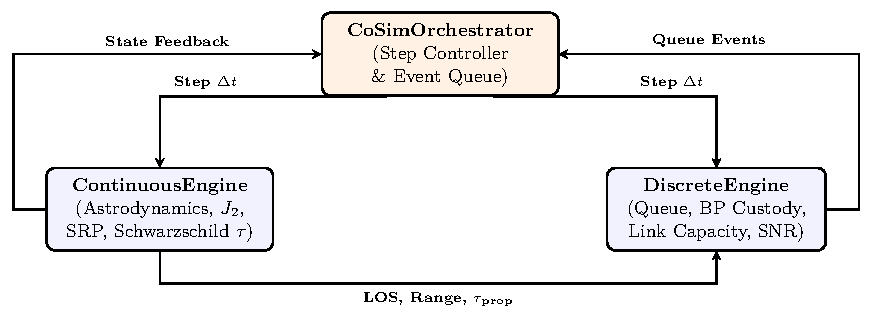
\includegraphics[width=\textwidth,height=0.40\textheight,keepaspectratio]{else_paper/fig_architecture.pdf}\\[2pt]
        {\footnotesize \textbf{Flight Engine (Continuous)} $\;\longleftrightarrow\;$ \textbf{Network Engine (ns-3)}}
      \end{tcolorbox}
    \end{column}

    \begin{column}{0.50\textwidth}
      \begin{tcolorbox}[colback=lightCyan,colframe=electricCyan!80!black,title=\textbf{Smart Step Controller: Zoom In \& Zoom Out}]
        \small
        \begin{itemize}\setlength{\itemsep}{1.5pt}
          \item \textbf{In Quiet Cruise:} Takes large strides in time (up to 1 hour) to run simulations at blazing speed.
          \item \textbf{Near Critical Events:} Automatically zooms in to split-second precision right as a satellite enters or leaves planetary shadow.
          \item \textbf{Zero Boundary Delay:} Catches every contact start and end with \textbf{0.0 ms error} without burning CPU time.
        \end{itemize}
      \end{tcolorbox}

      \vspace{1.5pt}
      \begin{tcolorbox}[colback=lightGreen,colframe=greenAccent,title=\textbf{True Time-Weighted Accuracy},top=1.5pt,bottom=1.5pt]
        \small
        Measures real orbital error across continuous mission time rather than artificially favoring fixed snapshots.
      \end{tcolorbox}
    \end{column}
  \end{columns}
\end{frame}

% -----------------------------------------------------------------------------
% Slide 4: Real-World Evidence Across Three Space Missions
% -----------------------------------------------------------------------------
\begin{frame}{Benchmark Proof: Faster, Lighter, and Exact}
  \begin{columns}[T]
    \begin{column}{0.46\textwidth}
      \begin{tcolorbox}[colback=white,colframe=spaceNavy,title=\textbf{Accuracy vs. Compute Effort},top=1.5pt,bottom=1.5pt]
        \centering
        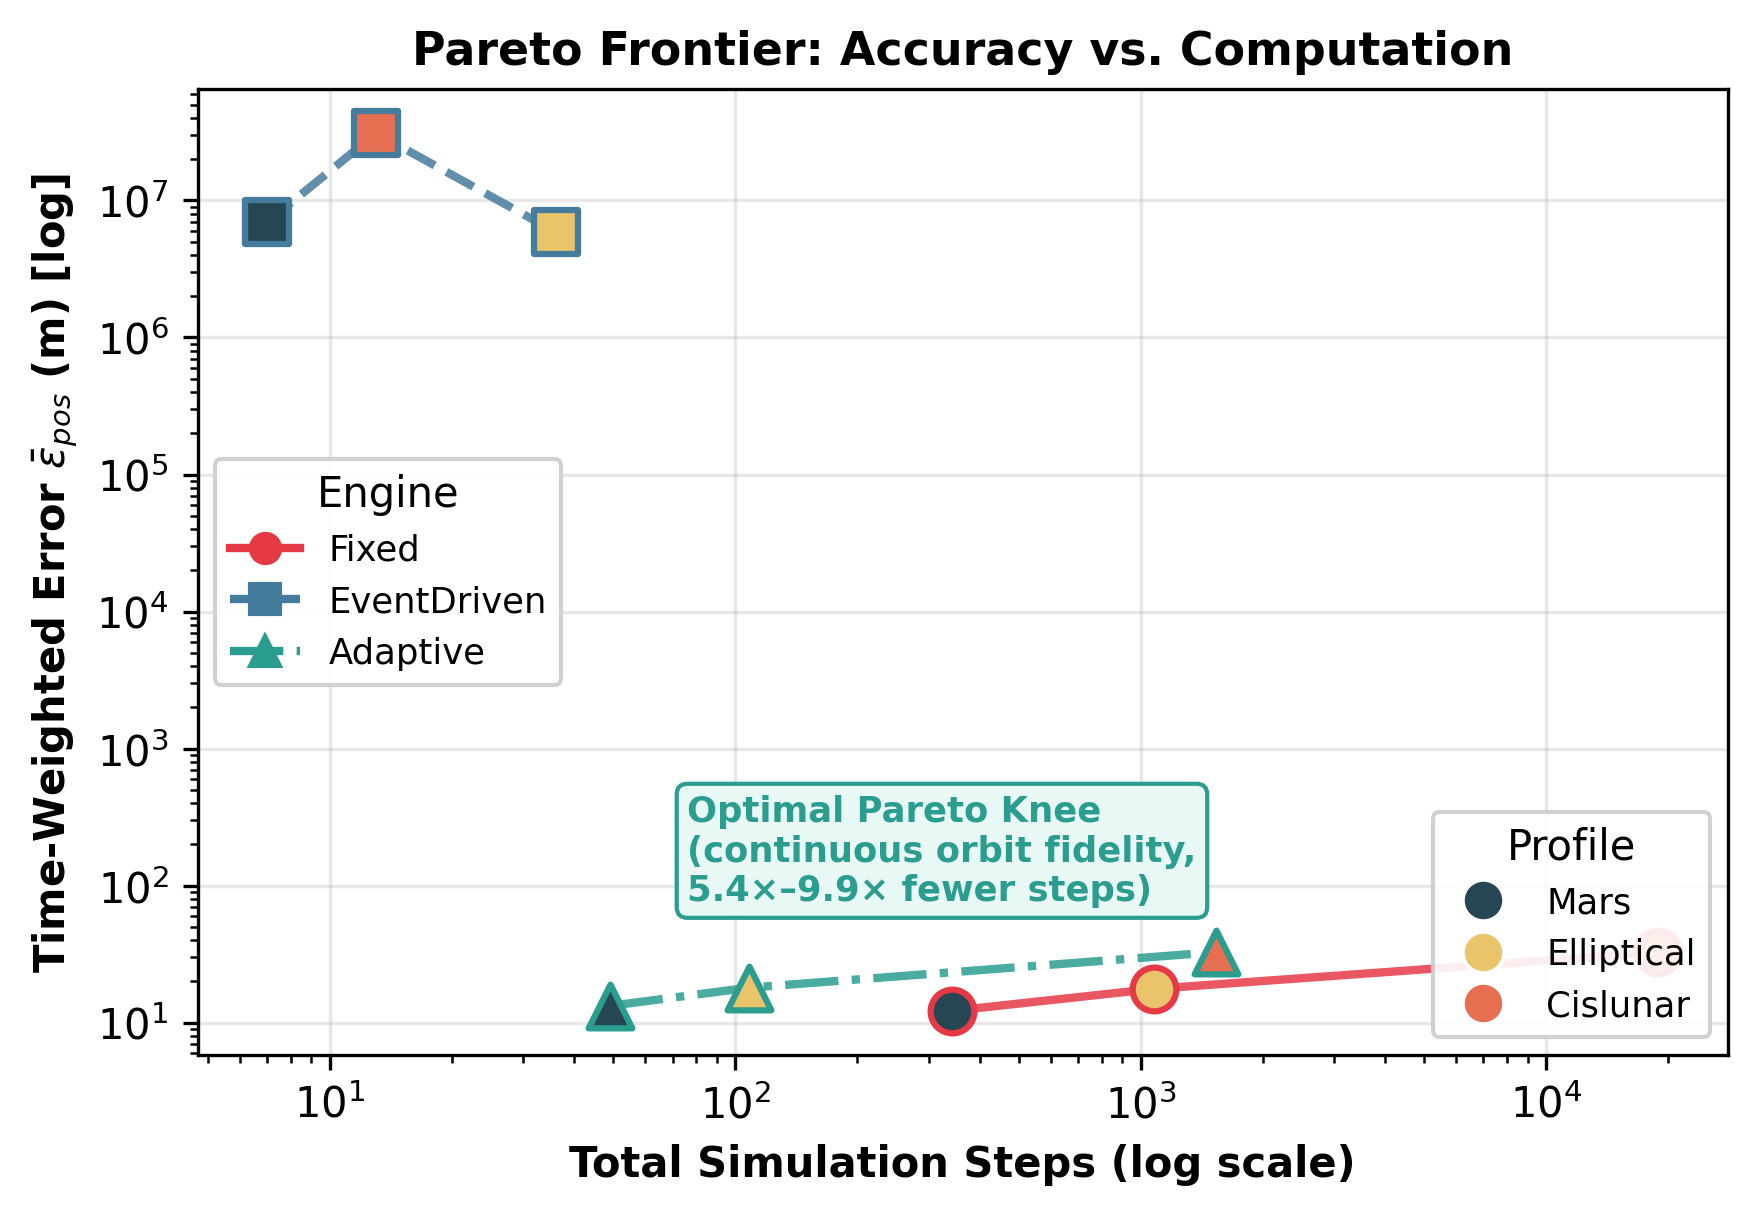
\includegraphics[width=\textwidth,height=0.43\textheight,keepaspectratio]{simulation/graphs/fig3_pareto_clean.png}\\[2pt]
        {\footnotesize\color{spaceNavy} \textbf{Optimal Knee:} 5x to 10x fewer computation steps with zero loss in orbital fidelity.}
      \end{tcolorbox}
    \end{column}

    \begin{column}{0.52\textwidth}
      \begin{tcolorbox}[colback=cardBg,colframe=spaceNavy,title=\textbf{Tested on 3 Realistic Mission Profiles},top=1.5pt,bottom=1.5pt]
        \small
        \begin{itemize}\setlength{\itemsep}{1pt}
          \item \textbf{Mars Occultation:} Passing behind the red planet.
            \begin{itemize}\setlength{\itemsep}{0pt}
              \item Runs \textbf{5.4x faster} than fixed stepping.
              \item \textbf{0.0 ms timing error} (vs. 30 seconds late in fixed).
            \end{itemize}
          \item \textbf{Molniya Orbit:} High-speed flyby near Earth.
            \begin{itemize}\setlength{\itemsep}{0pt}
              \item Runs \textbf{8.1x faster}; trajectory stays within 18 meters.
            \end{itemize}
          \item \textbf{13-Day Moon NRHO:} Long lunar cruise.
            \begin{itemize}\setlength{\itemsep}{0pt}
              \item Runs \textbf{9.9x faster}, saving over 17,000 wasted steps.
            \end{itemize}
        \end{itemize}
      \end{tcolorbox}

      \vspace{1.5pt}
      \begin{tcolorbox}[colback=lightGreen,colframe=greenAccent,title=\textbf{Scalability (10 to 500 Spacecraft)},top=1.5pt,bottom=1.5pt]
        \footnotesize
        Simulates 500 space nodes in just 6.35 seconds with zero software lockups.
      \end{tcolorbox}
    \end{column}
  \end{columns}
\end{frame}

% -----------------------------------------------------------------------------
% Slide 5: The 30,000-Kilometer Ghost Satellite
% -----------------------------------------------------------------------------
\begin{frame}{The Ghost Satellite Problem: Drifting into Nowhere}
  \begin{columns}[T]
    \begin{column}{0.56\textwidth}
      \begin{tcolorbox}[colback=white,colframe=spaceNavy,title=\textbf{Position Drift Over Long Missions},top=1.5pt,bottom=1.5pt]
        \centering
        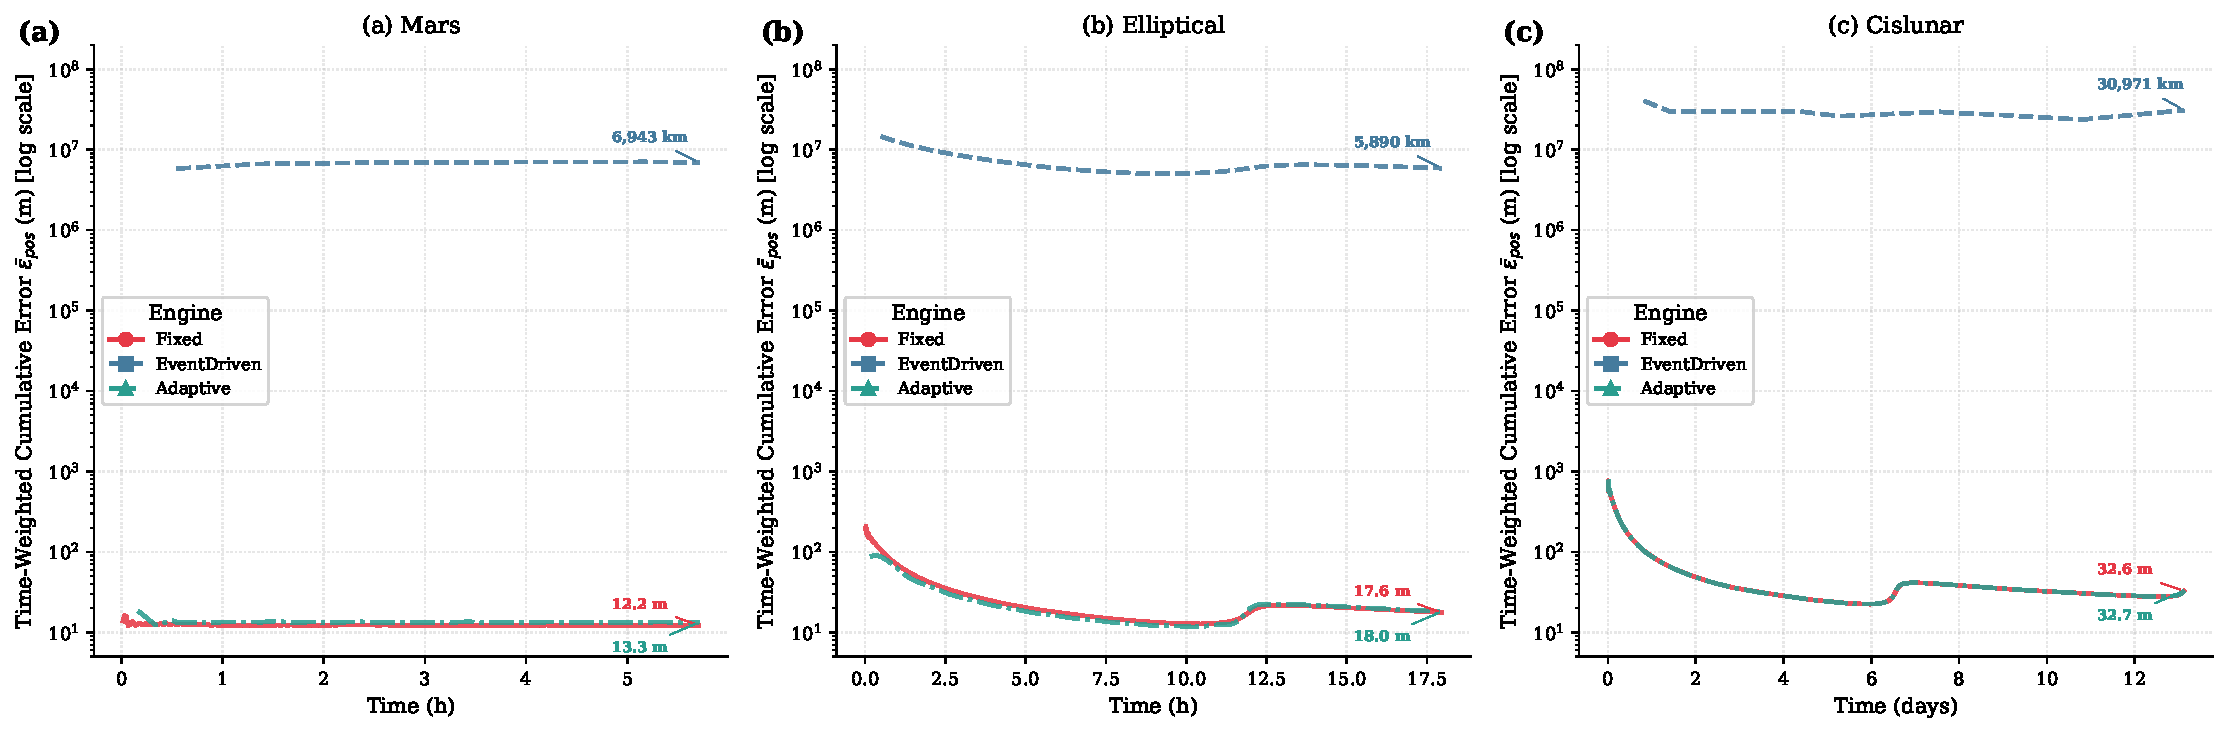
\includegraphics[width=\textwidth,height=0.48\textheight,keepaspectratio]{else_paper/fig5_cumulative_error.pdf}\\[2pt]
        {\footnotesize\color{spaceNavy} Pure event-driven DES explodes in error during radio silence; our adaptive engine stays flat on the real flight path.}
      \end{tcolorbox}
    \end{column}

    \begin{column}{0.42\textwidth}
      \begin{tcolorbox}[colback=lightRed,colframe=alertRed,title=\textbf{The Radio Silence Trap},top=1.5pt,bottom=1.5pt]
        \small
        \begin{itemize}\setlength{\itemsep}{1.5pt}
          \item When no radio packets are sent, traditional event simulators go completely blind.
          \item In our 13-day lunar mission, the simulated satellite drifts by \textbf{over 30,970 kilometers}!
          \item That is more than \textbf{double the diameter of Earth}!
        \end{itemize}
      \end{tcolorbox}

      \vspace{1.5pt}
      \begin{tcolorbox}[colback=lightGreen,colframe=greenAccent,title=\textbf{Our Adaptive Accuracy},top=1.5pt,bottom=1.5pt]
        \small
        \begin{itemize}\setlength{\itemsep}{1.5pt}
          \item Our engine continuously tracks real orbital gravity in the background.
          \item Maximum position drift is bounded to \textbf{meters}, perfectly matching NASA SPICE standards.
        \end{itemize}
      \end{tcolorbox}
    \end{column}
  \end{columns}
\end{frame}

% -----------------------------------------------------------------------------
% Slide 6: What Happens in the Real World If You Get This Wrong?
% -----------------------------------------------------------------------------
\begin{frame}{What Goes Wrong When Simulators Lie?}
  \begin{columns}[T]
    \begin{column}{0.49\textwidth}
      \begin{tcolorbox}[colback=lightRed,colframe=alertRed,title=\textbf{1. False Connection Predictions},top=1.5pt,bottom=1.5pt]
        \small
        \begin{itemize}\setlength{\itemsep}{0.8pt}
          \item A 30,000 km position error alters calculated radio signal strength by \textbf{up to 14 dB}.
          \item The simulator falsely reports a healthy high-speed link when the spacecraft is actually in \textbf{total radio blackout}.
        \end{itemize}
      \end{tcolorbox}

      \vspace{1.5pt}
      \begin{tcolorbox}[colback=lightGold,colframe=goldAccent,title=\textbf{2. Phantom Data Speeds},top=1.5pt,bottom=1.5pt]
        \small
        \begin{itemize}\setlength{\itemsep}{0.8pt}
          \item Modern radios adapt speed to signal quality.
          \item Stale positions cause the simulator to schedule peak data transmission (20 Mbps) when the actual channel is dead (0 Mbps).
        \end{itemize}
      \end{tcolorbox}
    \end{column}

    \begin{column}{0.49\textwidth}
      \begin{tcolorbox}[colback=lightCyan,colframe=electricCyan!80!black,title=\textbf{3. Panic Retransmission Storms},top=1.5pt,bottom=1.5pt]
        \small
        \begin{itemize}\setlength{\itemsep}{0.8pt}
          \item Deep space network timers rely on expected travel delay.
          \item Underestimating delay makes timers expire prematurely, triggering storms of duplicate packets that choke the network.
        \end{itemize}
      \end{tcolorbox}

      \vspace{1.5pt}
      \begin{tcolorbox}[colback=cardBg,colframe=spaceNavy,title=\textbf{4. Catastrophic Lost Science Data},top=1.5pt,bottom=1.5pt]
        \small
        \begin{itemize}\setlength{\itemsep}{0.8pt}
          \item Because the simulator claims data is flowing safely, mission planners do not realize onboard storage is overflowing.
          \item Precious scientific photos and telemetry are permanently deleted.
        \end{itemize}
      \end{tcolorbox}
    \end{column}
  \end{columns}

  \vspace{1.5pt}
  \begin{tcolorbox}[colback=cardBg,colframe=spaceNavy,top=1.5pt,bottom=1.5pt]
    \centering\footnotesize\color{spaceNavy}
    \textbf{The Golden Rule:} \textit{In deep space, a flight mechanics tracking error directly becomes a catastrophic networking failure.}
  \end{tcolorbox}
\end{frame}

% -----------------------------------------------------------------------------
% Slide 7: Three Actionable Upgrades for ns-3
% -----------------------------------------------------------------------------
\begin{frame}{Three Practical Blueprints for ns-3}
  \begin{tcolorbox}[colback=cardBg,colframe=spaceNavy,title=\textbf{Blueprint 1: Aim Where the Spacecraft Will Be (In-Flight Light Solver)},top=1.5pt,bottom=1.5pt]
    \small
    \begin{itemize}\setlength{\itemsep}{0.8pt}
      \item \textbf{Today's Limitation:} ns-3 calculates signal delay based on where the spacecraft was when the transmission started.
      \item \textbf{Our Proposal:} Teach ns-3 to solve where the moving target will actually be when the signal arrives minutes or hours later.
    \end{itemize}
  \end{tcolorbox}

  \vspace{1.5pt}
  \begin{tcolorbox}[colback=lightCyan,colframe=electricCyan!80!black,title=\textbf{Blueprint 2: Smart Early-Warning Alarms (Boundary Event Guarding)},top=1.5pt,bottom=1.5pt]
    \small
    \begin{itemize}\setlength{\itemsep}{0.8pt}
      \item \textbf{Today's Limitation:} Researchers force the computer to take millions of tiny steps just to watch for when a satellite dips behind a planet.
      \item \textbf{Our Proposal:} Introduce smart look-ahead triggers so the simulator speeds through quiet space and only slows down at the exact threshold crossings.
    \end{itemize}
  \end{tcolorbox}

  \vspace{1.5pt}
  \begin{tcolorbox}[colback=lightGold,colframe=goldAccent,title=\textbf{Blueprint 3: Deep-Space Multi-Clock Synchronization},top=1.5pt,bottom=1.5pt]
    \small
    \begin{itemize}\setlength{\itemsep}{0.8pt}
      \item \textbf{Today's Limitation:} ns-3 uses a single global clock that assumes time ticks identically everywhere.
      \item \textbf{Our Proposal:} Support local spacecraft clocks that adjust for Einstein's gravitational and speed time dilation near massive planets.
    \end{itemize}
  \end{tcolorbox}
\end{frame}

% -----------------------------------------------------------------------------
% Slide 8: Key Takeaways, Review Status & Open-Source Code
% -----------------------------------------------------------------------------
\begin{frame}{Key Takeaways \& Open-Source Code}
  \begin{columns}[T]
    \begin{column}{0.66\textwidth}
      \begin{tcolorbox}[colback=cardBg,colframe=spaceNavy,title=\textbf{What We Learned},top=1.5pt,bottom=1.5pt]
        \small
        \begin{itemize}\setlength{\itemsep}{1.5pt}
          \item Deep space breaks traditional network simulators: multi-minute delays and continuous flight cannot be treated as simple frozen events.
          \item Our adaptive engine runs \textbf{5x to 10x faster} with \textbf{zero timing error} ($0.0$ ms) and sublinear scaling up to 500 nodes.
          \item Ready-to-implement blueprints to make ns-3 ready for the next era of interplanetary exploration.
        \end{itemize}
      \end{tcolorbox}

      \vspace{1.5pt}
      \begin{tcolorbox}[colback=lightCyan,colframe=electricCyan!80!black,title=\textbf{Full Manuscript Under Peer Review},top=1.5pt,bottom=1.5pt]
        \small
        \textit{``The Limits of Discrete-Event Synchronization in Interplanetary Network Simulation: A Critical Review of Co-Simulation Fidelity''}\\
        Submitted to \textbf{Simulation Modelling Practice and Theory (Elsevier)}.
      \end{tcolorbox}
    \end{column}

    \begin{column}{0.31\textwidth}
      \begin{tcolorbox}[colback=white,colframe=spaceNavy,title=\textbf{Scan for Code \& Paper},top=1.5pt,bottom=1.5pt]
        \centering
        
\includegraphics[width=0.66\textwidth]{qrcode_preprint.png}\\[2pt]
        {\tiny\texttt{github.com/PandiaJason/}\\\texttt{SPICE-ns-Project}}
      \end{tcolorbox}

      \vspace{-2pt}
      \centering
      {\scriptsize \textbf{Presenter:} Jason Pandian\\
      \texttt{pandiajason@gmail.com}}
    \end{column}
  \end{columns}
\end{frame}

\end{document}
